\subsection{Převody mezi jednotlivými tvary rovnice přímky}
\label{subsec:Conversions_between_line_forms}

Parametrické vyjádření, obecná rovnice i směrnicový tvar mohou
popisovat tutéž přímku. Při převodu se tedy nemění samotný geometrický
objekt, ale pouze způsob jeho zápisu.

Jednotlivé tvary poskytují různé informace. Z parametrického vyjádření
přímo získáváme bod přímky a její směrový vektor, z obecné rovnice
normálový vektor a ze směrnicového tvaru směrnici a průsečík s osou
$y$.

Převodem můžeme zvolit takový zápis přímky, který je pro danou úlohu
nejvýhodnější. Parametrické vyjádření je vhodné například při vytváření
bodů přímky, obecná rovnice při ověřování příslušnosti bodu nebo při
řešení soustav rovnic a směrnicový tvar při zkoumání směru přímky
a jejího vztahu ke grafu lineární funkce.

\subsubsection{Přehled jednotlivých tvarů rovnice přímky}
\label{subsubsec:Overview_line_forms}

Uvažujme přímku $p$ v rovině. Tři dosud zavedené způsoby jejího zápisu
můžeme shrnout následovně:

\begingroup
\renewcommand{\arraystretch}{1.7}
\[
\begin{array}{c|c|c}
    \text{způsob vyjádření}
    &
    \text{základní tvar}
    &
    \text{údaje, které přímo získáme}
    \\
    \hline
    \text{parametrické}
    &
    \begin{aligned}
        x&=x_A+t u_x,\\
        y&=y_A+t u_y,
        \qquad t\in\mathbb{R}
    \end{aligned}
    &
    A[x_A;y_A],\quad
    \vec{u}=(u_x;u_y)
    \\[4mm]
    \text{obecné}
    &
    ax+by+c=0
    &
    \vec{n}=(a;b)
    \\[2mm]
    \text{směrnicové}
    &
    y=kx+q
    &
    k,\quad Q[0;q]
\end{array}
\]
\endgroup

Parametrické vyjádření a obecná rovnice umožňují popsat každou přímku
v rovině. Směrnicový tvar lze použít pouze pro přímky, které nejsou
rovnoběžné s osou $y$.

\begin{remark}\label{rem:Uniqueness_line_forms}
    Parametrické vyjádření ani obecná rovnice přímky nejsou určeny
    jednoznačně. Tutéž přímku můžeme parametricky zapsat pomocí různých
    jejích bodů a různých rovnoběžných směrových vektorů. Také obecnou
    rovnici můžeme vynásobit libovolným nenulovým číslem, aniž bychom
    změnili množinu jejích řešení.

    Směrnicový tvar nesvislé přímky je naopak jednoznačný. Jestliže dvě
    rovnice
    \[
        y=k_1x+q_1
        \qquad\text{a}\qquad
        y=k_2x+q_2
    \]
    popisují tutéž přímku, potom musí platit
    \[
        k_1=k_2
        \qquad\text{a}\qquad
        q_1=q_2.
    \]
\end{remark}

Možné převody mezi jednotlivými tvary jsou znázorněny na obrázku
\ref{fig:Conversions_between_line_forms}.

\begin{figure}[H]
    \centering
    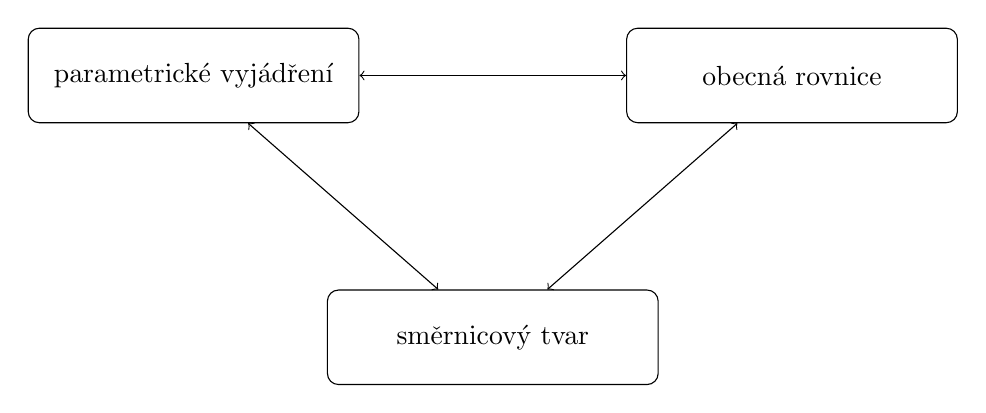
\begin{tikzpicture}[scale=0.95, every node/.style={align=center}]

        \node[
            draw,
            rounded corners,
            minimum width=4.2cm,
            minimum height=1.2cm
        ] (parametric) at (-4,1.5)
        {parametrické vyjádření};

        \node[
            draw,
            rounded corners,
            minimum width=4.2cm,
            minimum height=1.2cm
        ] (general) at (4,1.5)
        {obecná rovnice};

        \node[
            draw,
            rounded corners,
            minimum width=4.2cm,
            minimum height=1.2cm
        ] (slope) at (0,-2)
        {směrnicový tvar};

        \draw[<->] (parametric) -- (general);
        \draw[<->] (parametric) -- (slope);
        \draw[<->] (general) -- (slope);

    \end{tikzpicture}
    \caption{Převody mezi jednotlivými tvary rovnice přímky.}
    \label{fig:Conversions_between_line_forms}
\end{figure}


\subsubsection{Převod mezi parametrickým vyjádřením a obecnou rovnicí}
\label{subsubsec:Conversion_parametric_general}

\paragraph{Z parametrického vyjádření do obecné rovnice}

Uvažujme přímku zadanou parametricky ve tvaru
\begin{equation}\label{eq:Conversion_parametric_form}
    \begin{aligned}
        x&=x_A+t u_x,\\
        y&=y_A+t u_y,
        \qquad t\in\mathbb{R},
    \end{aligned}
\end{equation}
kde $A[x_A;y_A]$ je bod přímky a
\[
    \vec{u}=(u_x;u_y)
\]
je její nenulový směrový vektor.

K tomuto směrovému vektoru zvolíme kolmý normálový vektor
\[
    \vec{n}=(u_y;-u_x).
\]
Přímka prochází bodem $A[x_A;y_A]$, a proto můžeme použít rovnici
určenou bodem a normálovým vektorem:
\[
    u_y(x-x_A)-u_x(y-y_A)=0.
\]

Po roznásobení dostáváme
\begin{align*}
    u_yx-u_yx_A-u_xy+u_xy_A&=0,\\
    u_yx-u_xy+u_xy_A-u_yx_A&=0.
\end{align*}

Obecná rovnice přímky má tedy tvar
\begin{equation}\label{eq:Conversion_parametric_to_general}
    u_yx-u_xy+u_xy_A-u_yx_A=0.
\end{equation}

Její koeficienty můžeme zapsat jako
\[
    a=u_y,
    \qquad
    b=-u_x,
    \qquad
    c=u_xy_A-u_yx_A.
\]

Zvolili-li bychom opačně orientovaný normálový vektor
\[
    \vec{n}=(-u_y;u_x),
\]
získali bychom rovnici vynásobenou číslem $-1$. Obě rovnice by však
popisovaly tutéž přímku.

\begin{example}\label{exa:Conversion_parametric_to_general}
    Převeďte parametrické vyjádření přímky
    \[
        \begin{aligned}
            p:\quad x&=-2+3t,\\
                     y&=1+2t,
                     \qquad t\in\mathbb{R},
        \end{aligned}
    \]
    na obecnou rovnici.

    Z parametrického vyjádření získáme bod
    \[
        A[-2;1]
    \]
    a směrový vektor
    \[
        \vec{u}=(3;2).
    \]

    K němu zvolíme normálový vektor
    \[
        \vec{n}=(2;-3).
    \]

    Rovnici přímky zapíšeme pomocí bodu $A[-2;1]$ a normálového
    vektoru:
    \begin{align*}
        2(x-(-2))-3(y-1)&=0,\\
        2(x+2)-3(y-1)&=0,\\
        2x+4-3y+3&=0,\\
        2x-3y+7&=0.
    \end{align*}

    Obecná rovnice přímky je tedy
    \[
        p:2x-3y+7=0.
    \]

    Správnost můžeme ověřit například bodem odpovídajícím hodnotě
    $t=1$:
    \[
        P[1;3].
    \]
    Po dosazení do obecné rovnice dostáváme
    \[
        2\cdot1-3\cdot3+7=2-9+7=0.
    \]
\end{example}

\begin{remark}\label{rem:Eliminating_parameter_line_conversion}
    Parametr lze odstranit také přímým algebraickým postupem. Pokud
    například platí $u_x\neq0$, můžeme z první parametrické rovnice
    vyjádřit
    \[
        t=\frac{x-x_A}{u_x}
    \]
    a tento vztah dosadit do druhé rovnice.

    Postup pomocí normálového vektoru je však jednotný a funguje také
    pro vodorovné a svislé přímky, aniž bychom museli rozlišovat, která
    souřadnice směrového vektoru je nulová.
\end{remark}


\paragraph{Z obecné rovnice do parametrického vyjádření}

Uvažujme přímku zadanou obecnou rovnicí
\begin{equation}\label{eq:Conversion_general_form}
    ax+by+c=0,
    \qquad
    (a;b)\neq(0;0).
\end{equation}

Z koeficientů obecné rovnice získáme normálový vektor
\[
    \vec{n}=(a;b).
\]
Jako směrový vektor přímky můžeme zvolit například
\[
    \vec{u}=(-b;a).
\]

Dále potřebujeme určit alespoň jeden bod
\[
    A[x_A;y_A],
\]
který obecnou rovnici splňuje. Jeho souřadnice můžeme získat vhodnou
volbou jedné souřadnice a dopočítáním druhé.

Jakmile známe bod $A$ a směrový vektor $\vec{u}=(-b;a)$, dostáváme
parametrické vyjádření
\begin{equation}\label{eq:Conversion_general_to_parametric}
    \begin{aligned}
        x&=x_A-bt,\\
        y&=y_A+at,
        \qquad t\in\mathbb{R}.
    \end{aligned}
\end{equation}

\begin{example}\label{exa:Conversion_general_to_parametric}
    Převeďte obecnou rovnici
    \[
        q:3x-4y+5=0
    \]
    na parametrické vyjádření.

    Normálový vektor přímky je
    \[
        \vec{n}=(3;-4).
    \]
    Jako směrový vektor zvolíme
    \[
        \vec{u}=(4;3).
    \]

    Nyní určíme jeden bod přímky. Zvolíme například $x=1$:
    \begin{align*}
        3\cdot1-4y+5&=0,\\
        8-4y&=0,\\
        y&=2.
    \end{align*}

    Přímka tedy prochází bodem
    \[
        A[1;2].
    \]

    Parametrické vyjádření je
    \[
        \begin{aligned}
            q:\quad x&=1+4t,\\
                     y&=2+3t,
                     \qquad t\in\mathbb{R}.
        \end{aligned}
    \]

    Ověření provedeme dosazením parametrických rovnic do původní
    obecné rovnice:
    \begin{align*}
        3(1+4t)-4(2+3t)+5
        &=
        3+12t-8-12t+5\\
        &=
        0.
    \end{align*}

    Obecná rovnice je tedy splněna pro každé
    $t\in\mathbb{R}$.
\end{example}

\begin{remark}\label{rem:Choosing_point_general_to_parametric}
    Bod přímky můžeme určit různými způsoby. Je-li $b\neq0$, můžeme
    například položit $x=0$ a získat bod
    \[
        A\left[0;-\frac{c}{b}\right].
    \]
    Je-li $a\neq0$, můžeme položit $y=0$ a získat bod
    \[
        B\left[-\frac{c}{a};0\right].
    \]

    Někdy je však výhodnější zvolit jinou hodnotu souřadnice tak, aby
    výsledný bod měl celočíselné souřadnice.
\end{remark}


\subsubsection{Převod mezi obecnou rovnicí a směrnicovým tvarem}
\label{subsubsec:Conversion_general_slope}

\paragraph{Z obecné rovnice do směrnicového tvaru}

Uvažujme obecnou rovnici přímky
\[
    ax+by+c=0.
\]

Chceme-li ji převést do směrnicového tvaru, musíme z rovnice vyjádřit
proměnnou $y$. To je možné právě tehdy, když
\[
    b\neq0.
\]

Postupně dostáváme
\begin{align*}
    ax+by+c&=0,\\
    by&=-ax-c,\\
    y&=-\frac{a}{b}x-\frac{c}{b}.
\end{align*}

Porovnáním s rovnicí
\[
    y=kx+q
\]
získáme
\begin{equation}\label{eq:Conversion_general_to_slope}
    k=-\frac{a}{b},
    \qquad
    q=-\frac{c}{b}.
\end{equation}

\begin{example}\label{exa:Conversion_general_to_slope}
    Převeďte obecnou rovnici
    \[
        p:2x+3y-6=0
    \]
    do směrnicového tvaru.

    Vyjádříme proměnnou $y$:
    \begin{align*}
        2x+3y-6&=0,\\
        3y&=-2x+6,\\
        y&=-\frac{2}{3}x+2.
    \end{align*}

    Směrnicový tvar přímky je tedy
    \[
        p:y=-\frac{2}{3}x+2.
    \]

    Ze zápisu přímo získáme směrnici
    \[
        k=-\frac{2}{3}
    \]
    a průsečík s osou $y$
    \[
        P_y[0;2].
    \]
\end{example}


\paragraph{Ze směrnicového tvaru do obecné rovnice}

Uvažujme přímku ve směrnicovém tvaru
\[
    y=kx+q.
\]

Převedeme-li všechny členy na jednu stranu, dostáváme
\begin{equation}\label{eq:Conversion_slope_to_general}
    kx-y+q=0.
\end{equation}

Tato rovnice je obecnou rovnicí přímky. Obsahuje-li směrnice nebo
absolutní člen zlomky, můžeme celou rovnici vynásobit vhodným
nenulovým číslem a zlomky odstranit.

\begin{example}\label{exa:Conversion_slope_to_general}
    Převeďte směrnicový tvar
    \[
        q:y=-\frac{3}{4}x+2
    \]
    na obecnou rovnici.

    Převedeme všechny členy na levou stranu:
    \[
        \frac{3}{4}x+y-2=0.
    \]

    Abychom odstranili zlomek, vynásobíme celou rovnici číslem $4$:
    \[
        3x+4y-8=0.
    \]

    Obecná rovnice přímky je tedy
    \[
        q:3x+4y-8=0.
    \]

    Rovnice
    \[
        \frac{3}{4}x+y-2=0
    \]
    a
    \[
        3x+4y-8=0
    \]
    jsou navzájem ekvivalentní, protože druhá vznikla vynásobením
    první rovnice nenulovým číslem $4$.
\end{example}


\subsubsection{Převod mezi parametrickým vyjádřením a směrnicovým tvarem}
\label{subsubsec:Conversion_parametric_slope}

\paragraph{Z parametrického vyjádření do směrnicového tvaru}

Uvažujme parametrické vyjádření
\[
    \begin{aligned}
        x&=x_A+t u_x,\\
        y&=y_A+t u_y,
        \qquad t\in\mathbb{R}.
    \end{aligned}
\]

Jestliže platí
\[
    u_x\neq0,
\]
není přímka svislá a její směrnice je dána poměrem souřadnic směrového
vektoru:
\[
    k=\frac{u_y}{u_x}.
\]

Přímka prochází bodem $A[x_A;y_A]$, a proto můžeme použít
bodově-směrnicový tvar
\[
    y-y_A=k(x-x_A).
\]

Po dosazení směrnice dostáváme
\[
    y-y_A
    =
    \frac{u_y}{u_x}(x-x_A),
\]
a tedy
\begin{equation}\label{eq:Conversion_parametric_to_slope}
    y
    =
    \frac{u_y}{u_x}x
    +
    y_A
    -
    \frac{u_y}{u_x}x_A.
\end{equation}

Z toho plyne
\[
    k=\frac{u_y}{u_x},
    \qquad
    q=y_A-\frac{u_y}{u_x}x_A.
\]

\begin{example}\label{exa:Conversion_parametric_to_slope}
    Vraťme se k přímce z příkladu
    \ref{exa:Conversion_parametric_to_general}:
    \[
        \begin{aligned}
            p:\quad x&=-2+3t,\\
                     y&=1+2t,
                     \qquad t\in\mathbb{R}.
        \end{aligned}
    \]

    Její směrový vektor je
    \[
        \vec{u}=(3;2),
    \]
    a proto je její směrnice
    \[
        k=\frac{2}{3}.
    \]

    Přímka prochází bodem $A[-2;1]$, takže
    \begin{align*}
        q
        &=
        y_A-kx_A\\
        &=
        1-\frac{2}{3}\cdot(-2)\\
        &=
        1+\frac{4}{3}\\
        &=
        \frac{7}{3}.
    \end{align*}

    Směrnicový tvar přímky je
    \[
        p:y=\frac{2}{3}x+\frac{7}{3}.
    \]

    Po vynásobení rovnice číslem $3$ a převedení všech členů na jednu
    stranu získáme
    \[
        2x-3y+7=0,
    \]
    což je stejná obecná rovnice jako v příkladu
    \ref{exa:Conversion_parametric_to_general}.
\end{example}


\paragraph{Ze směrnicového tvaru do parametrického vyjádření}

Uvažujme přímku
\[
    y=kx+q.
\]

Z jejího směrnicového tvaru přímo získáme bod
\[
    Q[0;q].
\]

Jako směrový vektor můžeme zvolit
\[
    \vec{u}=(1;k),
\]
protože při zvětšení souřadnice $x$ o jednu jednotku se souřadnice
$y$ změní o hodnotu $k$.

Parametrické vyjádření proto můžeme zapsat ve tvaru
\begin{equation}\label{eq:Conversion_slope_to_parametric}
    \begin{aligned}
        x&=t,\\
        y&=q+kt,
        \qquad t\in\mathbb{R}.
    \end{aligned}
\end{equation}

Obsahuje-li směrnice zlomek, můžeme směrový vektor vynásobit vhodným
nenulovým číslem a získat tak vektor s celočíselnými souřadnicemi.

\begin{example}\label{exa:Conversion_slope_to_parametric}
    Převeďte směrnicový tvar
    \[
        r:y=-\frac{3}{2}x+4
    \]
    na parametrické vyjádření.

    Přímka prochází bodem
    \[
        Q[0;4].
    \]

    Ze směrnice můžeme nejprve získat směrový vektor
    \[
        \vec{u}_1=\left(1;-\frac{3}{2}\right).
    \]
    Abychom odstranili zlomek, vynásobíme tento vektor číslem $2$:
    \[
        \vec{u}=(2;-3).
    \]

    Parametrické vyjádření přímky je tedy
    \[
        \begin{aligned}
            r:\quad x&=2t,\\
                     y&=4-3t,
                     \qquad t\in\mathbb{R}.
        \end{aligned}
    \]

    Ověření provedeme dosazením parametrických rovnic do směrnicového
    tvaru:
    \[
        -\frac{3}{2}(2t)+4=-3t+4,
    \]
    což je právě druhá parametrická rovnice.
\end{example}


\subsubsection{Svislé přímky při převodech}
\label{subsubsec:Vertical_lines_conversions}

Svislé přímky vyžadují při převodech zvláštní pozornost. Přímka
rovnoběžná s osou $y$ má rovnici
\begin{equation}\label{eq:Vertical_line_equation_conversion}
    x=d,
    \qquad d\in\mathbb{R}.
\end{equation}

V obecném tvaru ji můžeme zapsat například jako
\[
    x-d=0.
\]
Jejím normálovým vektorem je
\[
    \vec{n}=(1;0)
\]
a směrovým vektorem například
\[
    \vec{u}=(0;1).
\]

Parametrické vyjádření svislé přímky můžeme zapsat jako
\begin{equation}\label{eq:Vertical_line_parametric_conversion}
    \begin{aligned}
        x&=d,\\
        y&=t,
        \qquad t\in\mathbb{R}.
    \end{aligned}
\end{equation}

Směrnicový tvar však pro svislou přímku neexistuje. Ze směrového
vektoru $\vec{u}=(0;1)$ bychom totiž měli získat směrnici
\[
    k=\frac{u_y}{u_x}=\frac{1}{0},
\]
což není definováno. Stejně tak svislá přímka není grafem žádné funkce
$y=f(x)$, protože jedné hodnotě $x=d$ odpovídá nekonečně mnoho hodnot
$y$.

\begin{example}\label{exa:Vertical_line_conversion}
    Převeďte obecnou rovnici
    \[
        p:2x-6=0
    \]
    na ostatní možné tvary.

    Po vydělení rovnice číslem $2$ získáme
    \[
        x-3=0,
    \]
    tedy
    \[
        x=3.
    \]

    Přímka prochází například bodem $A[3;0]$ a má směrový vektor
    \[
        \vec{u}=(0;1).
    \]

    Její parametrické vyjádření je
    \[
        \begin{aligned}
            p:\quad x&=3,\\
                     y&=t,
                     \qquad t\in\mathbb{R}.
        \end{aligned}
    \]

    Směrnicový tvar této přímky neexistuje, protože přímka je
    rovnoběžná s osou $y$.
\end{example}

\begin{remark}\label{rem:Horizontal_line_all_forms}
    Vodorovné přímky tento problém nemají. Přímku
    \[
        y=d
    \]
    můžeme zapsat všemi třemi způsoby:
    \[
        \begin{aligned}
            &\text{parametricky:}
            &&
            x=t,\quad y=d,
            \qquad t\in\mathbb{R},\\
            &\text{obecně:}
            &&
            y-d=0,\\
            &\text{směrnicově:}
            &&
            y=0x+d.
        \end{aligned}
    \]
    Její směrnice je tedy $k=0$.
\end{remark}

\begin{example}\label{exa:Line_forms_conversion_summary}
    Je dána přímka parametrickým vyjádřením
    \[
        \begin{aligned}
            p:\quad x&=1+2t,\\
                     y&=-2+3t,
                     \qquad t\in\mathbb{R}.
        \end{aligned}
    \]

    \begin{enumerate}[label=\alph*)]
        \item Určete obecnou rovnici přímky.
        \item Určete její směrnicový tvar.
        \item Ze získaného směrnicového tvaru sestavte jiné
        parametrické vyjádření téže přímky.
        \item Ověřte, že obě parametrická vyjádření popisují tutéž
        přímku.
    \end{enumerate}

    \begin{enumerate}[label=\alph*), leftmargin=2em]

        \item \textbf{Obecná rovnice}

        Z parametrického vyjádření získáme bod
        \[
            A[1;-2]
        \]
        a směrový vektor
        \[
            \vec{u}=(2;3).
        \]

        K němu zvolíme normálový vektor
        \[
            \vec{n}=(3;-2).
        \]

        Rovnici určenou bodem a normálovým vektorem zapíšeme jako
        \begin{align*}
            3(x-1)-2(y-(-2))&=0,\\
            3(x-1)-2(y+2)&=0,\\
            3x-3-2y-4&=0,\\
            3x-2y-7&=0.
        \end{align*}

        Obecná rovnice přímky je
        \[
            p:3x-2y-7=0.
        \]

        \item \textbf{Směrnicový tvar}

        Z obecné rovnice vyjádříme proměnnou $y$:
        \begin{align*}
            3x-2y-7&=0,\\
            -2y&=-3x+7,\\
            y&=\frac{3}{2}x-\frac{7}{2}.
        \end{align*}

        Směrnicový tvar přímky je
        \[
            p:y=\frac{3}{2}x-\frac{7}{2}.
        \]

        Stejný výsledek můžeme získat přímo z parametrického
        vyjádření:
        \[
            k=\frac{3}{2}
        \]
        a
        \[
            q
            =
            -2-\frac{3}{2}\cdot1
            =
            -\frac{7}{2}.
        \]

        \item \textbf{Jiné parametrické vyjádření}

        Ze směrnicového tvaru přímo získáme bod
        \[
            B\left[0;-\frac{7}{2}\right].
        \]

        Směrnici
        \[
            k=\frac{3}{2}
        \]
        odpovídá například směrový vektor
        \[
            \vec{v}=(2;3).
        \]

        Jiné parametrické vyjádření téže přímky je proto
        \[
            \begin{aligned}
                p:\quad x&=2s,\\
                         y&=-\frac{7}{2}+3s,
                         \qquad s\in\mathbb{R}.
            \end{aligned}
        \]

        \item \textbf{Ověření ekvivalence}

        Původní a nové parametrické vyjádření používají stejný směrový
        vektor
        \[
            \vec{u}=\vec{v}=(2;3).
        \]

        Stačí tedy ověřit, že bod
        \[
            B\left[0;-\frac{7}{2}\right]
        \]
        leží na původní přímce. Z první parametrické rovnice získáme
        \[
            0=1+2t,
            \qquad
            t=-\frac{1}{2}.
        \]

        Pro tuto hodnotu parametru dostáváme z druhé rovnice
        \[
            y
            =
            -2+3\left(-\frac{1}{2}\right)
            =
            -2-\frac{3}{2}
            =
            -\frac{7}{2}.
        \]

        Bod $B$ tedy na původní přímce leží, a obě parametrická
        vyjádření proto popisují tutéž přímku.

        Ekvivalenci můžeme vyjádřit také substitucí
        \[
            s=t+\frac{1}{2}.
        \]
        Potom
        \begin{align*}
            2s
            &=
            2\left(t+\frac{1}{2}\right)
            =
            1+2t,\\
            -\frac{7}{2}+3s
            &=
            -\frac{7}{2}
            +3\left(t+\frac{1}{2}\right)\\
            &=
            -\frac{7}{2}+3t+\frac{3}{2}\\
            &=
            -2+3t.
        \end{align*}
    \end{enumerate}

    Všechny tři zápisy
    \[
        \begin{aligned}
            x&=1+2t,\\
            y&=-2+3t,
            \qquad t\in\mathbb{R},
        \end{aligned}
    \]
    \[
        3x-2y-7=0
    \]
    a
    \[
        y=\frac{3}{2}x-\frac{7}{2}
    \]
    tedy popisují tutéž přímku.
\end{example}
